\section{Pixel Processing Unit (PPU)}

Figure \ref{diagram:ppu_block} shows the high-level structure of the PPU. This is the second-generation architecture -- the previous version had a number of sprite and tile engines operating in parallel, with shared bus access. This was a mistake. Many of these units were idle much of the time, and they were stripped down to the minimum to meet strict area requirements; this in turn led to poor bus utilisation and a lack of flexibility. The second problem was partially solved by the Poker, but at the expense of high software complexity for common use cases (e.g. many sprites on screen). The high level goals of PPU2 are, in order of precedence:

\begin{enumerate}
\item Always Be Fetching
\item Avoid idle or duplicated base functional units (e.g. pixel unpacker) so that more expensive functions can be provided (e.g. random access to pixels)
\item Be highly programmable, and allow features to be combined in interesting ways
\item Serve the simple use cases (layered, tiled backgrounds with sprites) with minimum program complexity
\item Mario Kart: Super Circuit
\end{enumerate}

Fundamentally we are fetching pixels from memory (over a 16 bit bus on RISCBoy), and putting them on the screen in interesting orders. If we saturate the bus, and do not waste what we fetch, our performance is as good as it possibly can be.

\begin{figure}[H]
\centering
\caption{Pixel processing unit, block-level diagram}
\label{diagram:ppu_block}
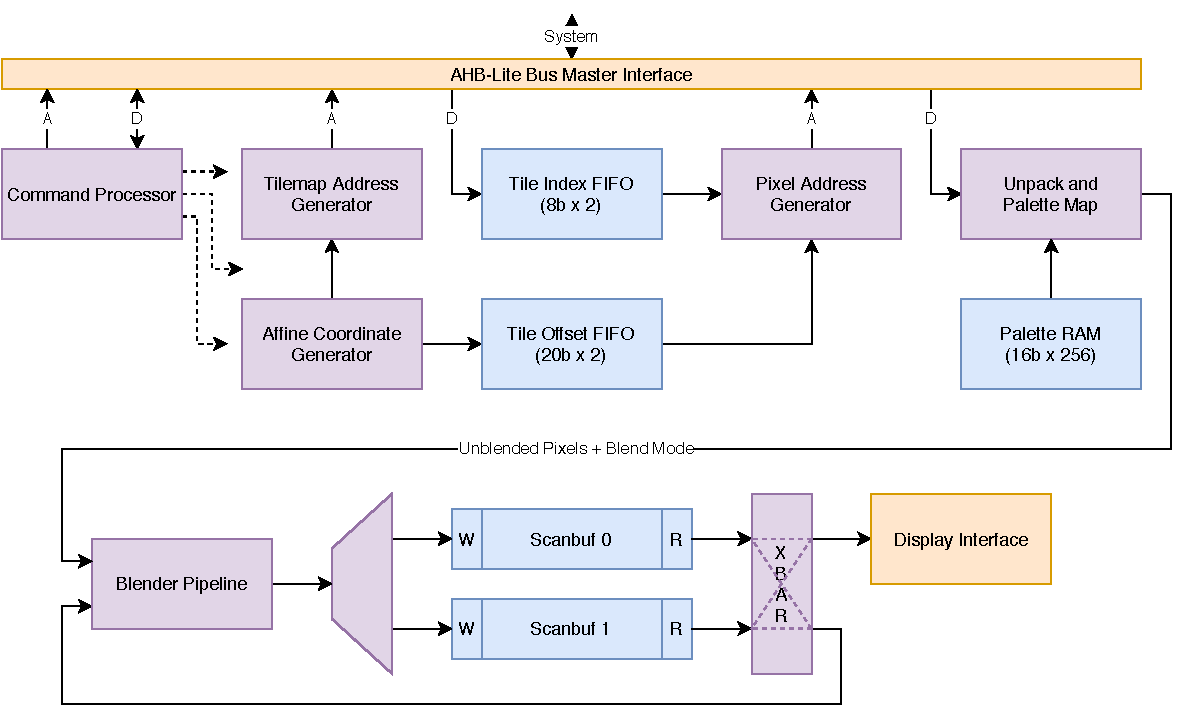
\includegraphics[width=\textwidth]{diagrams/ppu_block.pdf}
\end{figure}

At any point in time the PPU is either rendering to one of the internal scanline buffers, or waiting for a buffer to be freed and passed back by the display interface hardware. The exact sequence of operations the PPU performs while rendering is defined by a program in memory, executed by the command processor. The instruction set is small, and specialised to the task at hand -- for example the {\tt SYNC} instruction marks the current scanline buffer as ready for display, and waits for a buffer be freed by the display hardware, and the {\tt FILL} instruction writes a constant-colour span to some $x$ range of pixels.

Common memory access patterns (for nonpaletted pixels):

\begin{itemize}
	\item Sprite blitting: fetch a pixel from memory every cycle
	\item Tiling: fetch a tile index after every $n$ pixels, then $n$ pixel fetches
	\item Affine-mapped tiling: fetch tile indices and pixels on alternate cycles
\end{itemize}

The display interface is provides a simple handshake for acquiring/releasing dirty scanbuffers, routes read addresses from the display controller to the correct scan buffer, and routes data back. Currently two display controllers are available to connect to this interface: one for serial LCDs such as ILI9341, and another for direct DVI output. The PPU display interface is synchronous, and any clock crossing (to SCK domain for serial LCDs, or pixel clock domain for DVI) is handled inside the display controller.

\subsection{Pixel Formats}

Internally, the PPU uses a single native pixel format, namely ARGB 1555 (see figure \ref{diagram:pixformat}), but it can stream pixels from memory in a variety of formats, and convert internally. PPU memory accesses are \textbf{always little-endian}: for performance reasons the PPU performs the widest possible fetch, yielding multiple pixels each, which are numbered least-significant-first.

\begin{figure}[H]
\centering
\caption{PPU pixel formats}
\label{diagram:pixformat}
\begin{tabular}{r l}
	\raisebox{-1ex}[5ex][1.5ex]{
		\begin{bytefield}[endianness=big,bitformatting=\small, bitwidth=auto]{16}
		\bitheader{0,4,5,9,10,14,15} \\
		\bitbox{1}{A} \bitbox{5}{R} \bitbox{5}{G} \bitbox{5}{B}
		\end{bytefield}} & Mode 0: ARGB1555, alpha = 0 when transparent \\
		\\
	\raisebox{-1ex}[5ex][1.5ex]{
		\begin{bytefield}[endianness=big,bitformatting=\small, bitwidth=auto]{8}
		\bitheader{0,7} \\
		\bitbox{8}{Index}
		\end{bytefield}} & Mode 1: P8, an index into a table of 256 colours\\
		\\
	\raisebox{-1ex}[5ex][1.5ex]{
		\begin{bytefield}[endianness=big,bitformatting=\small, bitwidth=auto]{4}
		\bitheader{0,3} \\
		\bitbox{4}{Index}
		\end{bytefield}} & Mode 2: P4, an index into a table of 16 colours \\
		\\
	\raisebox{-1ex}[5ex][1.5ex]{
		\begin{bytefield}[endianness=big,bitformatting=\small, bitwidth=auto]{1}
		\bitheader{0} \\
		\bitbox{1}{I}
		\end{bytefield}} & Mode 3: P1, an index into a table of 2 colours \\
		\\
\end{tabular}
\end{figure}

For pixels smaller than one byte, the pixel order continues to be defined in a little-endian fashion, i.e. the least-significant pixel will be the first to be displayed. The PPU also requires image base addresses to be word-aligned, which implies all pixels are naturally aligned.

\subsection{Palettes}

The PPU contains a single hardware palette memory (PRAM), which is large enough to store 256 colours in ARGB1555 format. Each pixel in a paletted image (see figure \ref{diagram:pixformat}) consists of an index into PRAM. The PPU looks these indices up before passing pixels to the screen; wide colour range is maintained at reduced bits per pixel.

Since PRAM contents is in ARGB1555 format, there is no special convention for indicating whether a paletted pixel is transparent: the hardware always performs the palette lookup, and the resulting colour may or may not have its Alpha bit set.

Although there is only a single hardware palette, 256 colours in size, {\tt TILE} and {\tt BLIT} commands can supply an offset, which is added to each paletted pixel before palette lookup. PRAM may be initialised with e.g. multiple 16-colour tables at different (potentially overlapping) locations, giving effectively independent palettes.

PRAM can be written to (but not read) through the PPU's configuration interface.

\subsection{Scanline Buffers}


The scanline buffers are implemented as 1-read 1-write memories, which allows the blending pipeline to easily achieve a 1 pixel per clock throughput, keeping the bottleneck on the system bus. This could also be implemented as a double-width 1RW memory, but not a compelling tradeoff on FPGA.

\begin{figure}[H]
\centering
\caption{PPU scanline buffer states}
\label{diagram:ppu_buffer_states}
\includegraphics[width=0.7\textwidth]{diagrams/ppu_buffer_states.pdf}
\end{figure}

On RISCBoy these are 15b$\times512$ memories, each composed of a pair of iCE40 4~kb block RAMs. This is sufficient to store one QVGA RGB555 scanline in each buffer. The blitter and display pass each other buffers through a pair of queues, one containing clean buffers for the blitter, and the other containing dirty buffers for the display. After reset, both buffers are in the clean queue.

\subsection{Instruction Set}

\newcommand{\reservedfield}{\color{lightgray}\rule{\width}{\height}}

Each instruction consists of one or more words in memory; the blitter processes each instruction in turn, progressing in a linear fashion unless a {\tt JUMP} is encountered. This section describes the encoding of blitter instructions, and their operation. Some fields are marked as {\it reserved}, denoted by a grey colour fill in the bit diagrams. Reserved fields are not used by the current hardware, and should be written all-zeroes by software.

For simple purposes (e.g. tiled backgrounds with some sprites on top), the blitter can execute the same program on each scanline; the coordinate systems of {\tt BLIT}/{\tt TILE} commands take the current raster $y$ coordinate into account (see section \ref{section:coordinates}). However, the instruction set is quite flexible, and the blitter's features can be combined in interesting ways, with fancy-looking results.

\subsubsection*{SYNC}

\begin{bytefield}[endianness=big,bitformatting=\tiny]{32}
\bitheader{0,27,28,31} \\
\bitbox{4}{{\tt 0x0}} \bitbox{28}{\reservedfield} \\
\end{bytefield}

Present the current scanline buffer to the display, then stall until a clean buffer becomes available. If {\tt CSR\_HALT\_HSYNC} is set, or {\tt CSR\_HALT\_VSYNC} is set and this is the last line of the frame, halt the PPU.

\subsubsection*{CLIP}

\begin{bytefield}[endianness=big,bitformatting=\tiny]{32}
\bitheader{0,9,10,19,20,27,28,31} \\
\bitbox{4}{{\tt 0x1}} \bitbox{8}{\reservedfield} \bitbox{10}{{\tt x\_end}} \bitbox{10}{{\tt x\_start}} \\
\end{bytefield}

Set the active region for rendering. Pixels at $x$ coordinates less than {\tt x\_start} or greater than {\tt x\_end} will be unaffected by subsequent {\tt FILL}, {\tt [A]TILE} or {\tt [A]BLIT} operations. This region remains in effect until another {\tt CLIP} is executed.

Often it is sufficient to perform an initial {\tt CLIP} to the screen width, and never change from this value, but {\tt CLIP} has numerous applications when combined with pixel-filling operations: for example using {\tt CLIP} + {\tt ABLIT} pairs to render a sequence of short affine-textured spans.

\subsubsection*{FILL}

\begin{bytefield}[endianness=big,bitformatting=\tiny]{32}
\bitheader{0,4,5,9,10,14,15,27,28,31} \\
\bitbox{4}{{\tt 0x2}} \bitbox{13}{\reservedfield} \bitbox{5}{{\tt R}} \bitbox{5}{{\tt G}} \bitbox{5}{{\tt B}} \\
\end{bytefield}

Fill the entire clipped region with a single colour. Note that scanline buffers retain their old contents when passed back to the blitter by the display hardware; if you want a solid background colour, you must {\tt FILL} it into each scanline, or include it in your background tileset.

\subsubsection*{BLIT}

\begin{bytefield}[endianness=big,bitformatting=\tiny]{32}
\bitheader{0,9,10,19,20,21,22,24,25,27,28,31} \\
\bitbox{4}{{\tt 0x4}} \bitbox{3}{{\tt size}} \bitbox{3}{{\tt poff}} \bitbox{2}{\reservedfield} \bitbox{10}{{\tt y}} \bitbox{10}{{\tt x}} \\
\bitheader{0,1,2, 31} \\
\bitbox{30}{{\tt img}} \bitbox{2}{\tt fmt} \\
\end{bytefield}

Block image transfer: paste a square image (e.g. a sprite) over the current scanline. If this image does not intersect the current scanline due to its position and size, or if it is fully outside of the clipped region on this scanline, the {\tt BLIT} command has no effect, and completes immediately. Generally {\tt BLIT} is called on each scanline with the same arguments, to build up the full image. For example, each game sprite may correspond to a {\tt BLIT} command which runs on every scanline.

{\tt BLIT} also supports efficient framebuffer graphics: in this case each scanline will have a different {\tt BLIT} command with a {\tt y} equal to that scanline's position, and a {\tt img} pointer that is one scanline further advanced into a software framebuffer. This allows a framebuffer to be packed in memory as a flat $\textup{width} \times \textup{height}$ array of pixels.

\begin{itemize}
\item {\tt img} is a pointer to the source image, which is assumed to be word-aligned (hence the missing LSBs).
\item {\tt fmt} is the pixel format, as described in figure \ref{diagram:pixformat}. The values are: mode 0 ARGB1555, mode 1 P8, mode 2 P4, mode 3 P1.
\item {\tt size} defines the size of the source image: $\textup{width}=\textup{height}=2^{{\tt size} + 3}$, so square images from 8 to 1024 pixels are supported.
\item {\tt poff} is the palette offset. This is left-shifted by 5 and added to each paletted pixel, with wrap on overflow, before the pixel is looked up in the palette RAM.
\end{itemize}

\subsubsection*{TILE}

\begin{bytefield}[endianness=big,bitformatting=\tiny]{32}
\bitheader{0,9,10,19,20,21,22,24,25,26,27,28,31} \\
\bitbox{4}{{\tt 0x5}} \bitbox{2}{\reservedfield} \bitbox{1}{{\tt s}} \bitbox{3}{{\tt poff}} \bitbox{2}{\reservedfield} \bitbox{10}{{\tt yscroll}} \bitbox{10}{{\tt xscroll}} \\
\bitheader{0,1,2, 31} \\
\bitbox{30}{{\tt tilemap}} \bitbox{2}{{\tt pfs}} \\
\bitheader{0,1,2, 31} \\
\bitbox{30}{{\tt tileset}} \bitbox{2}{\tt fmt} \\
\end{bytefield}

Render a tiled background span (see section \ref{section:tiles}).

\begin{itemize}

\item {\tt xscroll} and {\tt yscroll} define the horizontal and vertical scroll of the tiled region. (TBD this may need to be redefined slightly for new PPU).

\item {\tt s} defines the size of the source image: $\textup{width}=\textup{height}=2^{{\tt s} + 3}$, so square images of $8\times 8$ or $16\times 16$ are supported.

\item {\tt poff} is the palette offset. This is left-shifted by 5 and added to each paletted pixel, with wrap on overflow, before the pixel is looked up in the palette RAM.

\item {\tt tileset} is a pointer to an array of $8\times 8$ or $16\times 16$~px images

\item {\tt fmt} is the pixel format of the tileset images, as described in figure \ref{diagram:pixformat}. The values are: mode 0 ARGB1555, mode 1 P8, mode 2 P4, mode 3 P1.

\item {\tt tilemap} is a pointer to a 2D array of 8 bit tile indices. Each index identifies which image from {\tt tileset} occupies that $8\times 8$ or $16\times 16$~px square.

\item {\tt pfs} is the playfield size in pixels, $\textup{width}=\textup{height}=2^{{\tt size} + 7}$, so 128 to 1024 px. See section \ref{section:tiles}.
\end{itemize}

\subsubsection*{ABLIT}

\begin{bytefield}[endianness=big,bitformatting=\tiny]{32}
\bitheader{0,9,10,19,20,21,22,24,25,27,28,31} \\
\bitbox{4}{{\tt 0x6}} \bitbox{3}{{\tt size}} \bitbox{3}{{\tt poff}} \bitbox{1}{\tt h} \bitbox{1}{\reservedfield} \bitbox{10}{{\tt y}} \bitbox{10}{{\tt x}} \\
\bitheader{0,15,16, 31} \\
\bitbox{16}{\tt b1} \bitbox{16}{\tt b0} \\
\bitheader{0,15,16, 31} \\
\bitbox{16}{\tt a01} \bitbox{16}{\tt a00} \\
\bitheader{0,15,16, 31} \\
\bitbox{16}{\tt a11} \bitbox{16}{\tt a10} \\
\bitheader{0,1,2, 31} \\
\bitbox{30}{{\tt img}} \bitbox{2}{\tt fmt} \\
\end{bytefield}


Like {\tt BLIT}, except screen coordinates are transformed before each pixel lookup:

\begin{align*}
\vec{u}   &= \vec{A}(\vec{s} - \vec{s}_0) + \vec{b} \\
\end{align*}

Where

\begin{align*}
\vec{u}   &= \begin{bmatrix}u & v \\ \end{bmatrix}^T & \textup{(texture coordinates)} \\
\vec{s}   &= \begin{bmatrix}s_x & s_y \\ \end{bmatrix}^T & \textup{(screen coordinates)} \\
\vec{s}_0 &= \begin{bmatrix}x & y \\ \end{bmatrix}^T & \textup{(blit target position {\tt x}, {\tt y})} \\
\vec{A}   &= \begin{bmatrix}a_{00} & a_{01} \\ a_{10} & a_{11} \end{bmatrix} & \textup{(scale/rotate/shear matrix)} \\
\vec{b}   &= \begin{bmatrix}b_0 & b_1 \\ \end{bmatrix}^T & \textup{(translation vector)} \\
\end{align*}

This affine transform is described in detail in section \ref{section:affine_transform}. It allows a range of geometric manipulations of the source image. {\tt ABLIT} renders to the same square region as {\tt BLIT}, defined by the {\tt size}, {\tt x} and {\tt y} parameters, as well as the current {\tt CLIP} region. It is the {\it texture lookup} for each rendered pixel that differs.

The {\tt a} components are signed 8.8 fixed point numbers, and {\tt b} components are unsigned 10.6 fixed point.
\begin{itemize}
	\item {\tt h}: half-size flag: indicate the texture is only half the size of the rasterized region in each axis. This allows e.g. a $32\times 32$~px texture to be rotated, without scaling, by \ang{45} and blitted to a $64\times64$~px region, so that its corners are not clipped. The effect of the half-size flag when {\tt size} = 0 is undefined.
	\item {\tt img} is a pointer to the source image, which is assumed to be word-aligned (hence the missing LSBs).
	\item {\tt fmt} is the pixel format, as described in figure \ref{diagram:pixformat}. The values are: mode 0 ARGB1555, mode 1 P8, mode 2 P4, mode 3 P1.
	\item {\tt size} defines the size of both the source image and the blit target area: $\textup{width}=\textup{height}=2^{{\tt size} + 3}$, so square images from 8 to 1024 pixels are supported.
	\item {\tt poff} is the palette offset. This is left-shifted by 5 and added to each paletted pixel, with wrap on overflow, before the pixel is looked up in the palette RAM.
\end{itemize}

\subsubsection*{ATILE}

\begin{bytefield}[endianness=big,bitformatting=\tiny]{32}
\bitheader{0,9,10,19,20,21,22,24,25,26,27,28,31} \\
\bitbox{4}{{\tt 0x7}} \bitbox{2}{\reservedfield} \bitbox{1}{{\tt s}} \bitbox{3}{{\tt poff}} \bitbox{2}{\reservedfield} \bitbox{10}{{\tt yscroll}} \bitbox{10}{{\tt xscroll}} \\
\bitheader{0,15,16, 31} \\
\bitbox{16}{\tt b1} \bitbox{16}{\tt b0} \\
\bitheader{0,15,16, 31} \\
\bitbox{16}{\tt a01} \bitbox{16}{\tt a00} \\
\bitheader{0,15,16, 31} \\
\bitbox{16}{\tt a11} \bitbox{16}{\tt a10} \\
\bitheader{0,1,2, 31} \\
\bitbox{30}{{\tt tilemap}} \bitbox{2}{{\tt pfs}} \\
\bitheader{0,1,2, 31} \\
\bitbox{30}{{\tt tileset}} \bitbox{2}{\tt fmt} \\
\end{bytefield}

Like {\tt TILE} but affine transform applied before each tile and pixel lookup: $\vec{u} = \vec{A}(\vec{s} - \vec{s}_0) + \vec{b}$. As with {\tt TILE}, the entire {\tt CLIP} region is rendered to. $\vec{s}_0$ is the {\tt xscroll}, {\tt yscroll} offset, the same as {\tt TILE}. All in all, {\tt TILE} can be thought of as a simple case of {\tt ATILE}, where $\vec{A}$ is the identity matrix and $\vec{b}$ is the zero vector.

\begin{itemize}
	\item {\tt s} defines the size of the source image: $\textup{width}=\textup{height}=2^{{\tt s} + 3}$, so square images of $8\times 8$ or $16\times 16$ are supported.
	\item {\tt poff} is the palette offset. This is left-shifted by 5 and added to each paletted pixel, with wrap on overflow, before the pixel is looked up in the palette RAM.
	\item {\tt tileset} is a pointer to an array of $8\times 8$ or $16\times 16$~px images
	\item {\tt fmt} is the pixel format of the tileset images, as described in figure \ref{diagram:pixformat}. The values are: mode 0 ARGB1555, mode 1 P8, mode 2 P4, mode 3 P1.
	\item {\tt tilemap} is a pointer to a 2D array of 8 bit tile indices. Each index identifies which image from {\tt tileset} occupies that $8\times 8$ or $16\times 16$~px square.
	\item {\tt pfs} is the playfield size in pixels, $\textup{width}=\textup{height}=2^{{\tt size} + 7}$, so 128 to 1024 px. See section \ref{section:tiles}.
\end{itemize}

\subsubsection*{PUSH}

\begin{bytefield}[endianness=big,bitformatting=\tiny]{32}
\bitheader{0,27,28,31} \\
\bitbox{4}{{\tt 0xe}} \bitbox{28}{\reservedfield} \\
\bitheader{0, 1, 2, 31} \\
\bitbox{30}{\tt data} \bitbox{2}{\reservedfield} \\
\end{bytefield}

Push literal {\tt data} onto the stack. The stack is popped only by a {\tt POPJ} instruction, is 8 words deep, and wraps on empty/full.

\subsubsection*{POPJ}

\begin{bytefield}[endianness=big,bitformatting=\tiny]{32}
\bitheader{0,9,10,23,24,27,28,31} \\
\bitbox{4}{{\tt 0xf}} \bitbox{4}{\tt cc}  \bitbox{14}{\reservedfield} \bitbox{10}{{\tt a}} \\
\end{bytefield}

Always pop an address from the stack. If {\tt cc} is true, branch to this address. Values for {\tt cc}:

\begin{itemize}
	\item 0: always
	\item 1: YLT, current raster beam $y < {\tt a}$
	\item 2: YNE, current raster beam $y \neq {\tt a}$
\end{itemize}

A regular jump is formed with {\tt PUSH addr; POPJ}, and a subroutine call is formed with {\tt PUSH ret; PUSH target; POPJ; label ret:} followed by a {\tt POPJ} at the end of the target routine.

Subroutines are useful for when a part of your command list is repeated every scanline (e.g. a list of sprites, represented by {\tt BLIT} commands) and a part is not (e.g. {\tt FILL}ing a different background colour every scanline to produce a gradient). Such a program can be structured as a larger per-frame command list which repeatedly calls into a per-scanline subroutine.


\subsection{Coordinate Systems}
\label{section:coordinates}

The origin of the screen is at the top left. $x$ coordinates increase to the right. $y$ coordinates increase going downward.


\begin{figure}[H]
\centering
\caption{PPU screen coordinate system}
\label{diagram:ppu_coord_screen}
\includegraphics[width=0.4\textwidth]{diagrams/ppu_coord_screen.pdf}
\end{figure}

When using a vector to refer to a screen-space coordinate, we will typically use the symbol $\vec{s}$.

\subsubsection*{Texture Coordinates}

\begin{figure}[H]
\centering
\caption{PPU texture coordinate system}
\label{diagram:ppu_coord_texture}
\includegraphics[width=0.25\textwidth]{diagrams/ppu_coord_texture.pdf}
\end{figure}

Textures (e.g. sprite images) have completely independent coordinates. We will conventionally refer to pixels in texture space with the vector $\vec{u} = \begin{bmatrix} u & v \\ \end{bmatrix}^T$. Textures are stored in memory as a flat array of pixels, going first in $u$ order and then stepping down to the next row.

When drawing a sprite, the PPU does the following:

\begin{itemize}
	\item Iterate over each pixel in some horizontal span of screen space
	\item For each pixel, transform the screen-space coordinate $\vec{s}$ into a texture-space coordinate $\vec{u}$
	\item Look up the texture pixel at $\vec{u}$ and draw it on the screen at $\vec{s}$
\end{itemize}

This transformation may be simple, as in the case of the {\tt BLIT} command:

\[
\vec{u} = \vec{s} - \vec{s}_0
\]

Where $\vec{s}_0$ is the position the texture is being blitted to ({\tt x}, {\tt y} in the {\tt BLIT} instruction), $\vec{s}$ is the position of next pixel to be rendered on the screen, and $\vec{u}$ is the position in texture space which determines the colour of the screen pixel. The transformation may be more complex, as in the case of the {\tt ABLIT} command:

\[
\vec{u} = \vec{A}(\vec{s} - \vec{s}_0) + \vec{b}
\]

Where the matrix $\vec{A}$ and vector $\vec{b}$ are constants supplied by the {\tt ABLIT} instruction, permitting any combination of translation, rotation, scale and shear. Note the direction of the definition: this is a mapping {\it from} screen space {\it to} texture space. If you find it more intuitive to think about mapping the texture onto the screen, you must note that this is the {\it inverse} of the above mapping, and you have some linear algebra to do.

Internally, the PPU represents $\vec{u}$-space coordinates as pairs of unsigned 10.8 fixed point numbers (a range of $0$ to $1023 + \frac{255}{256}$); the largest supported texture size is therefore $1024 \times 1024$~px.

As far as coordinates are concerned, there is no difference between e.g. a $512\times 512$~px texture and a $512\times 512$~px tiled background. The difference is that a texture's pixels are defined by a single large image ($512 \times 512$~px in this example), whereas the tiled area is defined by a number of small e.g. $16 \times 16$~px images called the {\it tileset}, and a 2D array of tile indices called the {\it tilemap} which defines which $16 \times 16$~px image should be at which $16 \times 16$~px region of $\vec{u}$-space.

\subsubsection*{Affine Transforms}
\label{section:affine_transform}

We gave the following definition for the transformation from screen space to texture space used by the {\tt ABLIT} and {\tt ATILE} commands:

\[
\vec{u} = \vec{A}(\vec{s} - \vec{s}_0) + \vec{b}
\]

All of our examples will use the following texture which, for argument's sake, is $64 \times 64$~px in size:

\begin{figure}[H]
\centering
\caption{PPU texture example}
\label{diagram:ppu_texture_example}
\includegraphics[width=0.25\textwidth]{diagrams/ppu_texture_example.pdf}
\end{figure}


Like {\tt BLIT}, {\tt ABLIT} renders to a square area of the screen, starting at $\vec{s}_0$ (defined by the {\tt x}, {\tt y} arguments to {\tt ABLIT}), and extending rightward and downward by the texture size.  If we set $\vec{A} = \vec{I} = \begin{bmatrix} 1 & 0 \\ 0 & 1 \\ \end{bmatrix}$ and $\vec{b} = \begin{bmatrix} 0 & 0 \\ \end{bmatrix}^T$, then the texture coordinate $\vec{u}$ is equal to the raster coordinate $\vec{s}-\vec{s}_0$, and the {\tt ABLIT} behaves the same as a {\tt BLIT}:

\begin{figure}[H]
\centering
\caption{PPU affine blit with identity mapping}
\label{diagram:ppu_texture_ablit01}
\includegraphics[width=0.8\textwidth]{diagrams/ppu_texture_ablit01.pdf}
\end{figure}

Setting $\vec{A}$ to the identity matrix maps the screen-space unit vectors $\vec{e}_x$ and $\vec{e}_y$ to the texture space's unit vectors $\vec{e}_u$, $\vec{e}_v$. The texture is undistorted. If we instead set $\vec{A} = \begin{bmatrix} 0 & 1 \\ 1 & 0 \\ \end{bmatrix}$:

\begin{figure}[H]
\centering
\caption{PPU affine blit with reflection in u=v}
\label{diagram:ppu_texture_ablit02}
\includegraphics[width=0.8\textwidth]{diagrams/ppu_texture_ablit02.pdf}
\end{figure}

The horizontal axis in screen space ($\vec{e}_x$) has instead been mapped to the vertical axis in texture space ($\vec{e}_v$), and vice versa. Texture lookups have been reflected across the line $u=v$.

We can perform a uniform scale by setting $\vec{A} = \lambda \vec{I}$, which maps the screen-space unit vectors onto {\it larger} vectors in texture space, so that texture samples of neighbouring screen pixels are further apart on the texture. E.g. take $\lambda=2$:

\begin{figure}[H]
\centering
\caption{PPU affine blit with uniform scale}
\label{diagram:ppu_texture_ablit03}
\includegraphics[width=0.8\textwidth]{diagrams/ppu_texture_ablit03.pdf}
\end{figure}

The $\vec{b}$ vector is used to translate texture lookups. It can be understood as the point in texture space to which the upper-left of the rasterised region is mapped, since at this point on the screen $\vec{s} = \vec{s}_0$, so $\vec{u} = \vec{A}(\vec{s}_0 - \vec{s}_0) + \vec{b} = \vec{b}$. For example, we could set $\vec{b} = \begin{bmatrix} -32 & -32 \\ \end{bmatrix}^T$, so that the sample corresponding to $\vec{s}_0$ is higher and further left in texture space:

\begin{figure}[H]
\centering
\caption{PPU affine blit with uniform scale and translation}
\label{diagram:ppu_texture_ablit04}
\includegraphics[width=0.8\textwidth]{diagrams/ppu_texture_ablit04.pdf}
\end{figure}

Figure \ref{diagram:ppu_texture_ablit04} shows $\vec{b}$ plotted in texture space, and the resulting shift of the sampled texture as seen in the rasterised area. For a final example, the matrix

\[
\vec{A} = \begin{bmatrix}
\cos\theta & -\sin\theta \\
\sin\theta & \cos\theta \\
\end{bmatrix}
\]

Defines, in our coordinate system, a clockwise rotation by $\theta$. Setting $\theta=45^{\circ}$, scaling by 2 and carefully choosing the $\vec{b}$ vector, we can make the texture appear to rotate {\it counterclockwise} about its centre in screen space.

\begin{figure}[H]
\centering
\caption{PPU affine blit with rotation}
\label{diagram:ppu_texture_ablit05}
\includegraphics[width=0.8\textwidth]{diagrams/ppu_texture_ablit05.pdf}
\end{figure}

Note that, without a scale factor, the corners of the texture would be clipped to the rasterised region of the screen. It is quite inefficient to take a large texture and always show it in a scaled-down form; {\tt ABLIT}'s half-size flag reduces the texture size to half of the rasterised region, so a $64\times 64$~px {\tt ABLIT} would expect a $32\times 32$~px texture, which would occupy the upper-left quadrant of the rasterised region if $\vec{A}=\vec{I}$ and $\vec{b}=\vec{0}$. This could then be rotated without scaling, and provided it is appropriately translated, the corners of the texture would not be clipped.

\subsection{Tiles}
\label{section:tiles}

To reduce memory footprint, the PPU is able to assemble scenes on the fly from an array of small images, known as tiles. TODO much of this section refers to old hw with dedicated tiled backgrounds engines

\begin{figure}[H]
\centering
\caption{PPU background coordinate system}
\label{diagram:ppu_bg_coords}
\includegraphics[width=0.7\textwidth]{diagrams/ppu_bg_coords.pdf}
\end{figure}

Each tile is a square image, the width and height of which (measured in pixels) is configured per-background, and is always a power of two. Tiles are stored as part of a larger image, known as the tileset. Tiles are numbered in a row-major order, starting at the top left of the tileset. An example tileset is shown in figure \ref{diagram:ppu_tileset}: this is a tileset of 8 tiles, each $4\times 4$ pixels in size.

\begin{figure}[H]
\centering
\caption{Example PPU tileset}
\label{diagram:ppu_tileset}
\includegraphics[width=0.7\textwidth]{diagrams/ppu_tileset.pdf}
\end{figure}

Each pixel row of the tileset is stored as a packed array of pixels in memory, and the next row follows. Note that all tiles must be the same size, and have the same pixel format.

The complete background image is assembled from these tiles. The arrangement is specified the tilemap: a grid of numbers, each naming a tile from the tileset. For each pixel on the screen, the tilemap tells the PPU which tile should be at that location, and the corresponding tile image in the tileset tells the PPU the colour of each pixel in that screen tile. This is shown in figure \ref{diagram:ppu_tilemap}.

\begin{figure}[H]
\centering
\caption{Example PPU tilemap}
\label{diagram:ppu_tilemap}
\includegraphics[width=0.7\textwidth]{diagrams/ppu_tilemap.pdf}
\end{figure}

The screen origin is offset into the background by configuring the horizontal and vertical scroll. This allows the game view to move smoothly over a fixed background. If the screen area overhangs the background, coordinates are wrapped.

In total, a background is defined by:

\begin{itemize}
	\item Width and height, measured in pixels
	\item Horizontal and vertical scroll, measured in pixels
	\item Tileset:
	\begin{itemize}
		\item Tile pixel format
		\item Tile size in pixels (power of two)
		\item Tileset width in pixels (power of two)
		\item Pointer to the tileset image (aligned to row size in bytes)
	\end{itemize}
	\item Tilemap:
	\begin{itemize}
		\item Pointer to the tilemap buffer
	\end{itemize}
\end{itemize}

This tilemapping process allows detailed images to be displayed with a minimal memory footprint, compared with a framebuffer, which must store the colour of every single pixel on the screen.
